\documentclass[a4paper,14pt]{extarticle}
\usepackage[utf8]{inputenc}
\usepackage[T2A]{fontenc}
\usepackage[russian]{babel}
\usepackage[left=2.5cm,right=1cm,top=2cm,bottom=2cm]{geometry}

\renewcommand{\rmdefault}{ftm}

\usepackage{color}
\usepackage[colorlinks,linkcolor=black,citecolor=black,urlcolor=black]{hyperref}
\renewcommand{\UrlFont}{\rmfamily}

\makeatletter
  \renewcommand{\@evenhead}{\vbox{\hbox to \textwidth {\hfil\thepage\hfil}}}
  \renewcommand{\@oddhead} {\vbox{\hbox to \textwidth {\hfil\thepage\hfil}}}
  \renewcommand{\@oddfoot} {\@empty}
  \renewcommand{\@evenfoot}{\@empty}
  
  \renewcommand{\maketitle}[5]{
    \def\@fletter{f}
    \def\@studentfemale{#3}
    \begin{titlepage}
      \begin{center}
        Министерство образования и науки Российской Федерации \\
        Федеральное государственное бюджетное образовательное учреждение \\
        высшего профессионального образования \\
        <<Волгоградский государственный технический университет>> \\
        Кафедра <<История, культура и социология>>
      \end{center}
      \vspace{9em}
      \begin{center}
        СЕМЕСТРОВАЯ РАБОТА \\
        ПО КУРСУ СОЦИОЛОГИИ \\
        ТЕМА №#1 \\
        \textbf{#2}
      \end{center}
      \vspace{3em}
      \begin{flushright}
        \begin{minipage}{.40\textwidth}
          \ifx\@studentfemale\@fletter
            \textbf{Выполнила:} \\
            студентка группы Ф-469 \\
          \else
            \textbf{Выполнил:} \\
            студент группы Ф-469 \\
          \fi
          #4 \\
          (№ зачётки #5) \\
          \vspace{1em} \\
          \textbf{Проверил:} \\
          Преподаватель кафедры ИКС \\
          доцент, кандидат соц.~наук \\
          Овчар~Н.~А.
        \end{minipage}
      \end{flushright}
      \vspace{\fill}
      \begin{center}
        Волгоград, \the\year
      \end{center}
    \end{titlepage}
    \global\let\@studentfemale\@empty
    \global\let\studentfemale\relax
    \global\let\@fletter\@empty
    \global\let\fletter\relax
  }
\makeatother

\usepackage{titletoc}
\titlecontents{section}[0em]{}{\contentslabel{1.75em}}{}
  {\titlerule*[1pc]{.}\contentspage}
\titlecontents{subsection}[0em]{}{\contentslabel{2.1em}}{}
  {\titlerule*[1pc]{.}\contentspage}
\titlecontents{subsubsection}[0em]{}{\contentslabel{2.5em}}{}
  {\titlerule*[1pc]{.}\contentspage}
  
\renewcommand{\thesection}      {\arabic{section}.}
\renewcommand{\thesubsection}   {\thesection\arabic{subsection}.}
\renewcommand{\thesubsubsection}{\thesubsection\arabic{subsubsection}.}

\usepackage{setspace}

\usepackage{titlesec}
\titleformat{\section}{\bf\normalsize\center}
  {Глава \thesection\hspace*{-5pt}} {1em}{\vspace{-.5em}}{}
\titleformat{\subsection}{\bf\normalsize\center}
  {\thesubsection\hspace*{-10pt}}   {1em}{\vspace{-.5em}}{}
\titleformat{\subsubsection}{\bf\normalsize\center}
  {\thesubsubsection\hspace*{-10pt}}{1em}{\vspace{-.5em}}{}


\begin{document}
  \maketitle{95}{СОВРЕМЕННЫЙ КОСТЮМ КАК СОЦИОКУЛЬТУРНЫЙ КОД ВРЕМЕНИ}
    {f}{Слоква~В.~И.}{20091236}
  \onehalfspacing
  \setcounter{page}{2}
  \tableofcontents

  \newpage

  \section*{Введение}
  \addcontentsline{toc}{section}{Введение}
  
  Социологи полагают, что одежда человека~-- такой же социальный сигнал, как и
  его речь, поведение и~т.~д. Даже те, кто уверяет, что <<наряды им совершенно
  не интересны>>, и одеваются настолько небрежно, насколько это возможно, по
  сути, таким образом сообщают о своей роли в обществе и о своем отношении к
  той культуре, в которой они живут.
  
  Влияет ли одежда на сознание современного общества, их поведение и отношение
  к другим индивидуумам? Моя работа посвящена поиску ответа на этот вопрос. В
  настоящее время существует понятие мода, но некоторые считают очень важным
  собственный <<стиль>> самовыражения. В связи с неоднозначным мнением на этот
  счет, я считаю что вопрос о связи социологии с одеждой является вполне
  актуальным.
  
  Цель моей работы выявить имеет ли одежда влияние на сознание современного
  общества. Для того, чтобы ответить на данный вопрос необходимо решить ряд
  задач: рассмотреть историю костюма и его значимость в разные значимые эпохи
  человечества, рассмотреть как относятся к одежде современные люди, как
  общественное мнение относительно вещей влияет на отдельных индивидов.
  
  Теоретической основой для моей работы стала книга Гофмана~А.~Б. <<Мода и
  люди. Новая теория моды и модного поведения>>, а также статьи журнала
  <<Социология и социальная антропология>>.
  
  Объектом исследований является одежда и мода. Предметом исследований является
  отношение человека к одежде и ее влияние на общественное сознание.
  
  Работа имеет практическую значимость в области социологии, маркетинга, среди
  дизайнеров и имиджмейкеров.
  
  Работа состоит из содержания, введения, пяти глав, заключения и списка литературы.
  
  \section{Определение понятия костюм, мода}
    
  История моды~-- составная часть истории материальной и духовной культуры и
  всеобщей истории искусств. Костюм синтезирует в себе различные виды
  прикладного искусства~-- ткачества, кружевоплетения, ювелирного дела,
  вышивки, орнаментации и~т.~д. Развитие этого наиболее массового вида
  творчества происходит под воздействием природно-–географической и
  предметно-–пространственной среды, социально--экономических изменений в
  жизни общества, национальных особенностей и межэтнических культурных
  контактов.

  Одежда в гораздо большей степени, чем остальное вещественное окружение людей
  (дом, мебель, предметы интерьера), представляет непосредственный символ
  индивидуального существования определенной группы, нации или целой эпохи.
  Костюм характеризует и дополняет картину общества на каждом этапе его
  развития. Почти каждый катаклизм в истории человечества вызывал значительные
  перемены в одежде.
  
  Природа костюма двояка: с одной стороны, он возник как рукотворный предмет
  утилитарного назначения, с другой~-- обладает своим идейно--образным
  содержанием, обусловленным многообразием функций одежды, мировоззрением и
  мировосприятием народа. Зримая знаковая структура костюма включает материал,
  крой, силуэт, колористику, орнаментику, способы ношения и комплектования
  деталей костюма, а также макияж, прическу и даже мимику, выразительные жесты
  и позы владельца костюма. Эти знаки вызывают образные ассоциации и эмоции,
  отражают половые и возрастные особенности, социальное, имущественное,
  семейное положение и место проживания человека, его магические, религиозные,
  эстетические представления.
 
  В изучении истории моды следует различать понятия <<одежда>> и <<костюм>>,
  <<исторический костюм>> и <<национальный костюм>>.
  
  Одежда~-- искусственный покров тела человека, защищающий его от
  неблагоприятных внешних воздействий природы и являющийся некоторым
  проявлением индивидуальности человека.
  
  Костюм~-- образно решенный ансамбль, который объединяет одежду, обувь,
  прическу, макияж, аксессуары и несет определенную эстетическую функцию.
  
  Каждый народ в любую историческую эпоху вырабатывал свою систему символов,
  которые с течением времени эволюционировали под влиянием культурных
  контактов, совершенствования технологии, расширения торговых связей. По
  сравнению с другими видами искусства костюм обладает еще одним важнейшим
  качеством~-- возможностью широко и почти мгновенно реагировать на события в
  жизни народа, на смену эстетических и идеологических течений в духовной
  сфере. Формы костюма всегда развиваются параллельно с развитием общего
  художественного стиля эпохи, переживая вместе с ним все этапы эволюции:
  зарождение, расцвет и угасание, причем с момента <<умирания>> старой, уже
  избившей себя костюмной формы начинается процесс формирования новой.
  
  В общепринятом смысле костюм часто ассоциируют с модой. История моды
  неразрывно связана с историей костюма, однако между ними нельзя ставить знак
  равенства, поскольку история костюма  началась вместе с историей первобытного
  общества, а мода, как социальное явление, появилась гораздо позже.
  
  Постоянное стремление человека к новизне заставляло создателей одежды
  беспрерывно искать новые формы и конструкции. С древнейших времен до
  настоящего времени с этим связана деятельность модельера--стилиста. Раньше
  художников, причастных к созданию костюма так не называли. Это были мастера
  по кружеву, вышивке, ремесленники, работающие над рисунками тканей, портные.
  Они создавали уникальные костюмы для узкого, избранного круга, которые
  входили в моду, завоевывали популярность у тысяч людей. Для настоящего
  времени характерна быстрая сменяемость модных циклов. Признаком процесса
  развития моды является сезонная смена циклов весна--лето и осень--зима. В
  связи с этим наблюдается стремительное изменение модных тенденций,
  образование новых форм в одежде.
  
  Мода~-- это отражение индивидуальных качеств отдельной личности в социальном
  и моральном аспекте.~\cite{bib:0}
  
  \section{Функции костюма в различные исторические периоды}
  
  У одежды три основных функции: обеспечение комфорта, соблюдение приличий и,
  так сказать, <<демонстрационная>> функция. Обеспечение комфорта~-- это,
  конечно же, внеобщественная и внеличностная функция одежды. Природа требовала
  от человека защищаться от жары, холода и~т.~д.
  
  Однако благодаря современной технологии люди, получается, могли бы отказаться
  от этой функции одежды: квартиры снабжены центральным отоплением и мягкой
  мебелью, так что мы можем преспокойно существовать в пределах своих квартир и
  без одежды. Но то, что мы этого не делаем, подводит нас к следующей основной
  функции одежды~-- к соблюдению приличий.
  
  В различные эпохи правила скромности были различными, но основной принцип
  оставался неизменным: чем более пуританским было общество, тем тщательнее
  полагалось скрывать свое тело. Пример крайности в этом отношении~-- одеяния
  женщин в некоторых арабских странах, где скрывается не только тело, но и
  его очертания. В этих странах женщина никогда не появлялась на людях без
  плотной вуали, и только ее муж знал, кто она на самом деле~-- красавица или
  <<чудовище>>.
  
  Сегодня трудно и представить, насколько далеко цивилизованное общество
  заходило в своих требованиях соблюдения приличий. Когда-то в Англии
  считалось непристойным даже произносить слово <<нога>>, а ножки роялей во
  время публичных концертов закрывались чехлами. Ступеньки, ведущие из
  купальных кабин в море или реку, занавешивались, чтобы посторонние не могли
  видеть, как люди в купальных костюмах спускаются в воду,-- и так было всего
  сто лет назад.
  
  Следующая функция одежды~-- демонстрационная. Запрет мужчинам появляться без
  галстука в дорогих ресторанах связан не с тем, что они обнажают адамово
  яблоко, а с тем, что галстук~-- это показатель определенного социального
  статуса. Как и многие другие элементы костюма, галстук выступает не как
  средство создания комфорта или в качестве детали, что-то скрывающей, а как
  знак, определяющий принадлежность его владельца к четкой социальной группе.
  И эта древнейшая функция одежды сохраняет свою значимость и в наши дни.
  Именно поэтому бесцветные, сугубо практичные туники людей космической эры,
  знакомые нам по второразрядным научно-фантастическим книгам и фильмам, так же
  маловероятны, как и возвращение человека к полной наготе. Как только общество
  отказывается от одного набора декоративных деталей одежды, на смену ему
  приходит новый~-- и подобная эволюция будет продолжаться, вероятно, до тех
  пор, пока человек не перестанет быть <<общественным животным>>: одежда~--
  слишком удобное средство для демонстрации статуса и взглядов ее обладателя,
  поэтому навряд ли человек откажется от этой ее функции и перейдет к
  нейтральной защитной оболочке.
  
  В прошлом демонстрационная функция одежды регламентировалась крайне жестко.
  Например, в Англии XIV века костюм определялся не вкусом или стилем, а
  законом. Большую часть времени тогдашний парламент посвящал определению
  правил одежды для каждого социального класса. Если человек надевал костюм,
  который полагался людям, стоящим выше его на общественной лестнице, он
  подвергался штрафу, а <<незаконная>> одежда конфисковалась. Однако закону
  этому люди сопротивлялись с упорством чрезвычайным: настолько велико было
  желание англичан демонстрировать~-- хотя бы посредством костюма~-- высокое
  положение в обществе. Правила ужесточались, штрафы росли~-- но тщеславие
  было непобедимо.
  
  Англия не была одинока в строгости. В Германии времен Возрождения женщина,
  нарушившая подобные правила, была обязана носить на шее тяжелый деревянный
  воротник. А в американских колониях женщине возбранялось носить шелковый
  шарф, если ее муж <<стоил>> меньше тысячи долларов.
  
  Все это~-- отдельные примеры, взятые из множества подобных предписаний,
  существовавших в ранние периоды истории человечества. Важно обратить внимание
  на следующее: люди стремились <<завысить>> свое положение в обществе, надевая
  <<не свой>> костюм, а наказывали их, по сути, не за сам костюм, но за попытку
  с его помощью завысить свой статус. В нашей обыденной жизни ношение одежды уже
  не ограничено такими жесткими правилами, тем не менее майор, например, не
  имеет права носить форму полковника, да и другие виды официального костюма
  регулируются столь же жестко, как и в давние времена.
  
  Может показаться, что современный <<распад>> системы <<костюмных>> законов и
  правил приведет к декоративному хаосу, но это отнюдь не так. Общество вместо
  того, чтобы прийти к полной свободе в выборе одежды, выработало свои
  собственные ограничения. Сначала юридические законы сменились законами
  этикета, сформулированными, пожалуй, не менее тщательно, чем уголовный
  кодекс. Затем, с уничтожением жесткой общественной структуры, пособия по
  этикету костюма исчезли. Но сами правила отнюдь не самоустранились~-- они
  просто <<ушли в подполье>>, став неписаными и даже не произносимыми вслух.
  Когда британского лорда спросили, есть ли преимущества в его общественном
  положении, он ответил: <<Есть только одно преимущество~-- я не должен
  одеваться так же чертовски тщательно, как мои слуги>>.
  
  Впрочем, свято место пусто не бывает: демонстрация своего высокого положения
  в обществе нашла новые формы. Так, например, в XVIII веке такой формой
  стал спорт. <<Высокородные>> мужчины занимались <<высокородными>> видами
  спорта. И при верховой езде английские сельские джентльмены надевали для
  удобства фраки и цилиндры~-- именно это одеяние стало ассоциироваться с
  досугом и возможностью не работать. <<Благородный>> спортивный костюм при
  помощи молодых модников превратился в повседневный костюм высшего света, а
  позже, к середине XIX века, стал обычным костюмом большой части
  общества.
  
  Но повседневность данного костюма лишила его признаков <<высокого статуса>>,
  и в поисках авангардных идей модники продолжали исследовать новую~--
  спортивную~-- сферу. Наступила очередь ружейной охоты, рыбалки и гольфа~--
  дорогостоящих развлечений, распространенных среди обеспеченных классов и
  потому являющихся прекрасным источником новых идей в области моды.
  Джентльмены надели клетчатые костюмы и котелки. Вначале подобная одежда
  считалась крайне неофициальной, но затем клетчатая ткань потеряла свою
  яркость и, став более приглушенной по цвету, вытеснила черный фрак, оставив
  ему скромное место одеяния для свадебных и других официальных торжеств, а
  также для некоторых вечерних <<мероприятий>>. И по сути, все без исключения
  современные деловые люди носят варианты костюмов, ранее являвшихся
  спортивными.
  
  В последние годы наметилась новая тенденция. Общество равных возможностей со
  все большей неприязнью относится к привилегиям, и это заставило тех, кто
  занимает высокое положение, еще более изощренно демонстрировать свой
  социальный статус. Стало немодным и даже опасным заявлять~-- при помощи
  одежды~-- о своей принадлежности к элите, которая может дозволить себе
  <<дорогие>> виды спорта. На смену <<клубному>> пиджаку яхтсмена пришла
  одежда, заимствованная у представителей общественных <<низов>>,~-- она
  давала возможность продемонстрировать, что в груди у богатых и знаменитых
  людей билось сердце <<простых парней>>.
  
  Самым первым симптомом таких перемен стала мода, родившаяся в результате
  отдыха в средиземноморских странах. Богатые молодые люди нарядились в грубые
  рубашки и свитеры местных рыбаков, затем мода распространилась во всех
  странах. Но какую, если вдуматься, информацию сообщала нам эта <<простая>>
  одежда непростых людей? А вот какую: <<Я одобряю бедных ребят, но сам к ним
  не отношусь>>. Как это им удается? Способов много. Первый~-- носить свитер и
  джинсы в тех общественных ситуациях, в которых бедняк оденется в свой лучший
  костюм. Второй~-- носить прекрасно сшитую, стилизованную <<одежду бедняка>>.
  Есть еще с десяток способов, но суть их одна~-- контраст между одеждой и тем,
  кто ее носит. Любой богатый или известный человек, чье лицо регулярно
  появляется на страницах газет и журналов, на экранах телевизоров и
  кинотеатров, может позволить себе надевать самую <<бедняцкую>> одежду на
  самые ответственные мероприятия. В этих случаях он или она, используя этот
  контраст, совершает молчаливую, но активную атаку на общество, превозносящее
  благосостояние в качестве высшей ценности.

  \begin{table}[t!]
    \center
    \small
    \caption{Эволюция социологических концепций моды}
    \label{tab:1}
    \begin{tabular}{|*{2}{C{.2}|C{.15}|}C{.17}|} \hline
      Концепция (теоретики) & <<Золотой век>> концепции & Социальная сущность
        моды & Способ создания образца & Лидеры моды, референтные группы
        \\ \hline
      Подражание (Тард, Спенсер, Зиммель) & До начала XX века &
        Подражание высшему классу & Образец создается персонально &
        Аристократия, элита \\ \hline
      Демонстративное потребление (Зомбарт, Веблен) & До середины
        XX века & Демонстративное потребление & Образец создается
        обезличенно (индустрией) & Богемные слои среднего класса \\ \hline
      Обновление социокультурных норм (Блумер) & До конца XX века &
        Функция социокультурного обновления & Образец создается плюралистично
        (многими референтными группами) & Журналы мод, модельеры и манекенщицы,
        поп-звезды, звезды спорта, молодежь \\ \hline
      Индустрия моды & С конца XX века & Симуляция общества & Образец
        создается виртуально (мир моды) & Виртуальные референтные группы
        (подиум, телевидение, журналы) \\ \hline
    \end{tabular}
    
    \medskip
    Источник: Ятина,~Л.~И. Мода глазами социолога: результаты
      эмпирического исследования~/ Л.~И.~Ятина~// Журнал социологии и
      социальной антропологии, том I.~-- 1998.~-- №~2.~-- С.~120--131.
  \end{table}
  
  В сложном мире сигналов, <<излучаемых>> человеческой одеждой, существует
  множество тенденций. Часто они пересекаются, одни из них быстротечны, другие
  живут десятилетиями. Кратковременные тенденции~-- это обычно не более чем
  поиск нового; в их основе лежит потребность носителей одежды демонстрировать
  свою <<современность>>. Такие тенденции зачастую быстро облетают земной шар
  и затем уходят в небытие. Однако демонстрация последних тенденций моды
  свидетельствует не только о том, что индивидуум идет в ногу с обществом, но и
  о его способности через определенные интервалы времени платить за новую
  модную одежду, то есть о его социальном статусе. Следя за мельчайшими
  изменениями в деталях нашего костюма (например, за изменениями ширины брюк
  или пиджачных лацканов), можно составить графики изменений сигналов,
  подающихся человеческой одеждой. Бессознательно мы постоянно составляем такие
  графики, что помогает нам <<считывать>> множество сигналов, передаваемых нам
  другими людьми. Таким образом, одежда является такой же частью языка
  человеческого общения, как и жесты, выражения лица и позы.~\cite{bib:2}

  \section{Семь социальных функций моды}
  \subsection{Функция создания и поддержания единообразия и разнообразия в
    культурных образцах}
    
  Единообразие и разнообразие можно рассматривать как две стороны одной и той
  же функции моды. В зависимости от критерия различения этих двух сторон, от
  фазы модного цикла и особенностей взаимодействия моды и социальной системы на
  первый план выдвигается унифицирующая или дифференцирующая функция моды.
  
  Функцию единообразия в конце 60-х годов предложил известный американский
  социолог и социальный психолог Г.~Блумер в <<Международной энциклопедии
  социальных наук>>. Единообразие проявляется в том, что благодаря моде один и
  тот же культурный образец (художественный стиль, фасон одежды, материал,
  размер и~т.~д.) усваивается и принимается в качестве своего множеством
  индивидов, различными социальными группами и глобальными обществами. Наивысшая
  степень единообразия достигается на высшей фазе модного цикла, когда данный
  культурный образец, оказавшийся <<в моде>> (модный стандарт), охватывает
  максимум приверженцев. Поддерживаемое модой единообразие, как справедливо
  отметил Блумер, играет важную позитивную роль, обеспечивая согласие в
  современных условиях, когда различные культурные образцы конкурируют между
  собой. К этому можно добавить, что модное единообразие способствует
  взаимопониманию и развитию контактов между глобальными обществами, а это
  сегодня насущнейшая проблема.
  
  Именно за порождаемое ею единообразие моду часто критикуют, обвиняя ее в
  повсеместной стандартизации и утверждении одинаковых вкусов. По этому поводу
  следует заметить, что без определенной степени единообразия в культурных
  образцах, в образе жизни, в повседневном поведении социальная жизнь вообще
  была бы невозможна. Некоторые ратуют за то, чтобы каждый индивид <<творчески>>
  подходил к проблемам повседневной жизни и самостоятельно решал, что и когда
  ему носить, что приобретать из домашней обстановки и~т.~д. Если такие люди
  абсолютно уверены в том, что сами, ни на кого и ни на что не ориентируясь,
  выбрали себе костюм и шляпу, если они каждый день вновь и вновь творчески
  решают вопрос о том, как оригинально держать вилку, то, как говорится, дай им
  Бог. В реальной же жизни нормальный индивид осуществляет свой выбор из
  образцов, предлагаемых обществом, под влиянием общества и социальных групп.
  Некоторые интериоризованные, усвоенные культурные образцы, регулирующие
  бытовую жизнедеятельность, превращаются в повседневные привычки, носят
  автоматический характер и отнюдь не требуют мобилизации творческого потенциала
  личности, высвобождая его для решения более серьезных задач.
  
  Демонстративный отказ от стандартов, предписываемых модой, чаще всего означает
  предпочтение других стандартов, предписываемых либо обычаем, либо прежними
  <<модами>>. Точка зрения, согласно которой <<раньше>>,~т.~е. при господстве
  обычая, однообразия в культурных образцах было меньше, в значительной мере
  основана на недоразумении. Несомненно, с планетарной точки зрения разнообразия
  в культурных образцах, присущих различным регионам, обществам, сословиям,
  этническим и конфессиональным группам и общинам, было больше. Но сама
  планетарная точка зрения тогда была невозможна: это мы, люди сегодняшнего дня,
  с этой позиции хотим и можем оценивать степень единообразия (разнообразия)
  культурных образцов. Что же касается самих этих групп и общин, то внутри
  каждой из них существование человека было в высокой степени унифицировано
  каноническим культурным стандартом~-- обычаем.
  
  Специфичность каждой из общин базировалась на отсутствии связей между ними, на
  их взаимной географической, социальной и культурной изолированности и
  замкнутости. Своеобразие их бытия находилось в неразрывной связи с его
  единообразием.
  
  Вернемся, однако, к моде. Каждый отдельно взятый модный стандарт в
  определенный промежуток времени формирует единообразие среди его приверженцев.
  Но одновременно и наряду с ним сосуществуют и другие модные стандарты:
  старомодный, которому еще следуют, и сверхмодный, которому уже следуют. И
  <<старомодное>>, и <<сверхмодное>> также относятся к моде: ведь все это звенья
  в единой и непрерывной цепи модного процесса. Стало быть, однообразие,
  формируемое отдельными <<модами>>, сочетается с разнообразием, порождаемым
  модой как социокультурным процессом в целом.
  
  Кроме того, как уже отмечалось выше, вследствие социальной, экономической и
  культурной дифференциации модный стандарт неодинаков в различных группах, он
  дробится на ряд модификаций. Одна и та же <<мода>> зачастую проявляется в
  бесчисленном множестве вариантов, например определенный вид промышленных
  изделий различных классов, из разных материалов, с разным набором функций
  и~т.~д. Самое же главное, и это следует еще раз подчеркнуть, одним и тем же
  <<модам>> в различных социальных и культурных средах приписываются самые
  различные значения, они связываются с самыми разнообразными ценностями, и в
  этом смысле <<унифицирующая>> мода также играет дифференцирующую роль.
  
  Необходимо обратить внимание на еще один аспект функции
  единообразия--разнообразия, обычно игнорируемый исследователями моды.
  Известно, что современное массовое поточное производство основана на
  унификации и стандартизации как процессов, так и результатов этого
  производства. Условием его эффективности является синхронизация определенных
  этапов, ритмов производства и его идентичных результатов. Однообразие в той
  или иной мере~-- неизбежный спутник массового производства. Но проблема
  единообразия-разнообразия имеет не только синхроническое, но и диахроническое
  измерение. Обновляя продукцию и соответствующие процессы ее создания и
  распространения, модные инновации производят диахронное,~т.~е.
  неодновременное, разнообразие. Осуществляя диахронное разнообразие, мода,
  таким образом, выполняет важную функцию компенсации синхронного однообразия,
  выступающего как условие и результат массового поточного производства.
  
  Применительно к социальным группам функция единообразия-разнообразия является
  в значительной мере функцией групповой демаркации-нивелирования посредством
  модных стандартов (<<мод>>). Этот вопрос был рассмотрен нами в предыдущей
  главе, что избавляет нас от необходимости вновь к нему обращаться.
  
  \subsection{Инновационная функция}

  Инновационная функция~-- одна из основных и наиболее очевидных функций моды:
  то, что мода несет с собой новизну, знает каждый. Поскольку действие моды
  распространяется на самые различные сферы социально-экономической и культурной
  жизни, постольку она увеличивает инновационный потенциал общества, готовность
  к внедрению и принятию нововведений в соответствующих сферах. Она влияет на
  обновление промышленной продукции, технологии, художественных стилей и~т.~д. В
  каждом обществе, социальной группе, в каждом секторе их жизнедеятельности
  существует определенная степень готовности к нововведениям~-- инновационности.
  Мода~-- источник, результат и показатель высокой степени инновационности.
  Поскольку ритм социально-экономической и культурной жизни неодинаков в
  различные периоды, постольку и степень инновационности одного и того же
  общества или группы изменяется.
  
  Стимулируя инновационность, мода способствует адаптации индивидов и
  общества к изменяющимся условиям их существования, как внутренним, так и
  внешним. Дело не в том, что все предлагаемые модой решения заведомо адекватны
  этим условиям. Основное значение имеет тот факт, что мода стимулирует
  эвристическое, поисковое, экспериментальное начало в обществе и культуре,
  развивает в социальной системе готовность не только к собственно модным, но и
  к другим видам нововведений.
  
  Усиливая инновационность общества или социальной группы, мода тем самым
  ослабляет его традиционность и подрывает власть обычая. Причем отказ от
  унаследованных культурных образцов в пользу новых в этом случае не связан с
  социальной дезинтеграцией, поскольку благодаря моде этот отказ санкционирован
  обществом и социальными группами.
  
  Однако взаимодействие инновационной функции моды с традиционными культурными
  образцами отнюдь не однозначно. Во-первых, эта функция иногда включается в
  традиционные образцы, ассимилируется ими. Простейший пример: фасоны брюк
  постоянно изменяются, обновляются, но ношение самих брюк как таковых
  традиционно и неизменно. Если первые относятся к сфере моды, то последнее
  принадлежит обычаю. <<Моды>> в данном случае функционируют в рамках обычая.
  
  Во-вторых, инновационная функция моды нередко выступает в форме актуализации
  культурной традиции. Время от времени модными значениями наделяются те или
  иные элементы культурного наследия. Дизайнеры широко используют в своем
  творчестве стилевые особенности традиционных культур как в одежде, так и в
  других областях. Так, Ив~Сен-Лоран в своих моделях часто опирается на
  традиционные черты русской, китайской, индийской, африканской, испанской
  одежды. Многие модели В.~Зайцева основаны на творческой интерпретации русской
  традиционной одежды.
  
  В наше время актуализация традиции широко распространена и представлена весьма
  разнообразно. Здесь и мода на <<старину>> и <<ретро-стили>> в различных видах
  искусства, и консервативные мифы о прошлом как <<золотом веке>>
  социокультурного бытия, и вспышки ксенофобии и~т.~д. О том, что в этих формах
  сознания сказывается влияние моды (хотя, разумеется, не только моды), говорит
  тот факт, что аналогичная актуализация традиции и традиционализма происходит
  одновременно в различных странах.
  
  В-третьих, некоторые культурные образцы, наделяемые модными значениями,
  первоначально выступающие как <<моды>> или даже причуды, со временем
  традиционализируются, превращаются в обычай. Так произошло, например, с такими
  <<модами>> или причудами былых времен, как вилка (XVIII~в.), велосипед
  (XIX~в.), авторучка (XX~в.).
  
  Или возьмем, например, наручные часы. Они появились в конце XIX~в. и вначале
  воспринимались многими как вульгарная и недолговечная диковинка. Еще в 1917~г.
  один немецкий профессор предсказывал: <<Глупая мода носить часы на руке скоро
  пройдет>>. Сегодня этот прогноз кажется странным и смешным, а в то время он
  выглядел вполне правдоподобно, тем более что наручным часам противостояли их
  старшие и солидные собратья~-– <<нормальные>> карманные часы. Первыми, как это
  нередко бывало в истории, на новинку клюнули <<легкомысленные>> женщины, столь
  часто вызывающие осуждение суровых моралистов. В 1914~г. большинство
  читательниц одного женского немецкого журнала своим любимым украшением назвали
  часы-браслеты. Затем достоинства наручных часов оценили любители верховой
  езды, автомобилисты, пилоты аэропланов и офицеры, участники первой мировой
  войны, оценившие преимущества наручных часов в боевой обстановке. В настоящее
  время в мире ежегодно выпускается около полумиллиарда наручных часов; былая
  мода превратилась в повсеместный обычай.
  
  Сегодня происходит традиционализация многих <<мод>>, причуд, диковинок и
  забав. Разумеется, модные стандарты традиционализируются сравнительно редко,
  но длительность модных циклов бывает все же весьма значительна. Отдельные
  <<моды>>, как бы ни были они летучи и преходящи, все же нельзя уподобить
  мыльным пузырям. Они обладают социальной и культурной длительностью, могут
  довольно долго сохраняться, а впоследствии возрождаться. Некоторые из них
  способны превращаться в устойчивые, традиционные культурные образцы. Стало
  быть, можно утверждать, что выполняемая модой функция инновации нередко
  способствует сохранению и возрождению культурных образцов.
  
  \subsection{Коммуникационная функция}  
  
  Все знаковые системы, функционирующие в обществе, служат средством
  коммуникации между людьми; мода~-- одна из таких систем. Коммуникация~-- одна
  из важнейших функций, без которой человеческое общество вообще невозможно.
  
  Подобно многим другим знакам, <<моды>> служат средством взаимодействия
  индивидов, социальных групп и обществ. Как уже отмечалось, модная коммуникация
  состоит в том, что от одних людей к другим передаются модные стандарты,
  <<моды>>,~т.~е. определенные культурные образцы, наделяемые модными
  значениями. Вместе с этими стандартами происходит передача обозначаемых ими
  ценностей моды: <<внутренних>> (современности, универсальности, игры и
  демонстративности) и стоящих за ними разнообразных <<внешних>> ценностей,
  выражающих глубинные потребности и стремления различных обществ, социальных
  групп и индивидов.
  
  Посредством участия в моде индивиды отправляют друг другу сообщения о своей
  приверженности ее ценностям, а также связывают их со своей группой, профессией
  и~т.~д. Эти сообщения выражают образ идеального Я участника моды. По данным
  социально-психологического исследования, 50 девушек в возрасте 15--16 лет,
  которым было предложено оценить рисунки современной одежды, представили
  последнюю прежде всего как средство сообщений о ее носителе. Высокая оценка
  определенной одежды связана со сходством этих сообщений с образом идеального Я
  субъекта и главным образом с ее модностью.
  
  В процессе распространения, восприятия и усвоения <<мод>> происходит их
  реинтерпретация в соответствии с собственными денотативными (<<внешними>>)
  ценностями воспринимающих эти <<моды>> обществ, групп и индивидов. Таким
  образом, <<моды>>, с одной стороны, усваиваются, с другой~-- модифицируются в
  зависимости от глубинных социальных, культурных и психических структур, в
  которые они включаются. Такое явление, впрочем, вообще характерно для
  распространения культурных образцов.
  
  Модная коммуникация специфична постольку, поскольку специфична сама мода как
  социальное явление. Наиболее существенными особенностями модной коммуникации
  являются сравнительно частая смена сообщений и их широкое, иногда практически
  безграничное распространение. Механизмы, способы и каналы коммуникации в моде
  в значительной мере совпадают с другими знаково-ценностными системами. Подобно
  другим культурным образцам, модные стандарты и ценности передаются как через
  непосредственное взаимодействие (речь, жесты, мимика и~т.~д.), так и через
  многообразные специальные средства межличностной и массовой коммуникации: от
  телефона до газеты и телевизора. В целом проблемы коммуникации многосторонне
  исследовались в социальных науках, поэтому здесь нет необходимости их
  специально рассматривать.
  
  Психологические аспекты коммуникации описываются в понятиях подражания,
  внушения, психического заражения, эмпатии, интериоризации социальных норм и
  ценностей. Межличностная коммуникация~-- <<условие психологической нормы>> и в
  реализацию этой нормы мода вносит определенный вклад. Модная коммуникация
  способствует формированию у индивидов согласия и общности в ценностных
  ориентациях.
  
  Социально-экономические и культурные аспекты коммуникации описываются
  преимущественно понятиями обмена, влияния, социального контроля, конкуренции,
  контактов, аккультурации (культурного заимствования) и~т.~д. Понятно, что
  социальная коммуникация в целом и модная в частности существенно затруднена в
  условиях существования разного рода <<железных занавесов>>, культурной
  изоляции, ксенофобии, психологической отчужденности и~т.~д. Перечисленные
  факторы вообще препятствуют нормальному функционированию и развитию культуры.
  Поскольку мода способствует социальным и культурным контактам, необходимым для
  нормального функционирования и развития обществ и культур, она выполняет
  позитивную социальную функцию.
  
  Чтобы быть успешной, модная коммуникация должна быть двусторонней и взаимной,
  а процессы социальной интериоризации культурных образцов необходимо сочетать с
  процессами их экстериоризации. Иными словами, движения сообщений <<извне>> и
  <<вовне>>, или, что то же самое, <<вовнутрь>> и <<изнутри>>, социальной
  системы должны идти рядом друг с другом. Кроме того, необходимо, чтобы
  усваиваемые <<моды>> гармонично сочетались с уже функционирующими в обществе
  фундаментальными ценностями. Определенные барьеры на пути заведомо негативных,
  антигуманных <<мод>>, несомненно, должны существовать, в противном случае
  коммуникация из функции моды может превратиться в дисфункцию.
  
  \subsection{Функция социальной дифференциации и нивелирования}
  
  Важное значение в осуществлении этой функции имеет время подключения тех или
  иных участников к определенному стандарту: на ранних фазах модного цикла
  доминирует дифференцирующая сторона этой функции, на высших фазах, когда
  стандарт охватывает большие массы людей,~-- нивелирующая сторона.
  
  Подобно унификации и разнообразию, дифференциацию и нивелирование уместно
  рассматривать не столько как две отдельные функции моды, сколько как два
  аспекта, две стороны одной и той же функции. Отсюда следует, что в конкретных
  исследованиях модного поведения главная проблема состоит не в том, чтобы
  доказать наличие дифференциации или нивелирования, а в том, чтобы показать,
  как в моде взаимодействуют оба эти процесса.
  
  И наконец, последняя важная констатация в связи с отмеченной функцией: мода в
  целом (а не отдельные <<моды>> в отдельные периоды) охватывает общество в
  целом. А это означает, что ее нельзя считать уделом ни элиты, ни отдельных
  социальных классов и слоев, демографических групп и~т.~д. Все они так или
  иначе принимают в ней участие, хотя формы участия и степень его активности,
  разумеется, неодинаковы.
  
  \subsection{Функция социализации}
  
  Мода~-- одно из средств приобщения индивида к социальному и культурному
  опыту,~т.~е. она выполняет функцию социализации.
  
  Участие в моде связано с усвоением определенных социальных норм и ценностей.
  По справедливому утверждению Т.~Б.~Любимовой, <<от других видов социализации
  мода отличается тем, что она обращена на общедоступные образцы>>. Этим она
  отличается от таких форм социализации, как образование или участие в
  профессиональной деятельности.
  
  Активное участие молодежи в моде отчасти объясняется социализирующей функцией
  этого явления: ведь именно в молодости происходит наиболее активное освоение
  социальных ролей, норм и ценностей. Важно не только содержание собственно
  модных стандартов, но и сам факт следования неким нормативным образцам,
  участие в социальной жизни как таковой. Это участие благодаря моде выступает в
  значительной мере в игровой и демонстративной формах, что облегчает процесс
  социальной адаптации.
  
  Хотя модные стандарты и ценности носят нормативный характер (как и любые
  другие средства социальной регуляции), степень императивности,
  принудительности, жесткости их предписаний не очень велика. Так называемый
  <<диктат>> моды зачастую преувеличивается в массовом и околопрофессиональном
  сознании. Это видно хотя бы из того факта, что нарушение нормативных
  предписаний моды, как правило, не влечет за собой серьезных социальных санкций
  по отношению к <<провинившемуся>>.
  
  С другой стороны, мода играет важную роль и в тех случаях, когда индивид
  испытывает потребность <<скрыть>> свое Я, раствориться среди других индивидов.
  Воспроизведение модного стандарта в период его наибольшей распространенности,
  привычности позволяет индивиду сделаться незаметным, раствориться среди других
  участников моды.
  
  Очевидно, мода~-- далеко не единственное и не главное средство личностного
  самоутверждения и самореализации. Тем большее значение она приобретает в этом
  качестве для тех индивидов, которые по тем или иным причинам или на том или
  ином этапе своего жизненного пути не находят иных средств.
  
  Активное участие в моде становится компенсацией иных социально
  санкционированных путей личностного самоутверждения. Если индивид не находит
  себя в профессиональной, творческой, социальной и других сферах, мода
  становится для него самодовлеющим способом утверждения своего Я и усиления его
  привлекательности для других.
  
  Особенно важна эта функция для индивидов с неустойчивой психикой, для которых
  собственное Я представляется проблематичным и нуждается в постоянном
  подтверждении своей реальности, устойчивости и привлекательности.
  
  Отсюда, в частности, опять-таки особая роль моды для молодежи. Молодой
  человек, еще не освоивший набор социальных ролей, еще формирующий свое
  самосознание и в известном смысле проектирующий свое Я, испытывает особенно
  острую потребность в социально санкционированных средствах личностной
  идентификации, одно из которых обеспечивает мода.
  
  Тем не менее не только молодежь, но и некоторые социально-психические типы
  личности особенно подвержены модной регуляции. Повышенная тревожность,
  неуверенность в себе, неустойчивость психологического и социального статуса
  усиливают зависимость от предписаний, исходящих от модных стандартов.
  Последние воспринимаются в этих случаях не просто как некие более или менее
  условные правила поведения и образцы культуры, а как жесткие нормы, нарушение
  которых самим <<нарушителем>> воспринимается как подлинная трагедия, а другими
  участниками моды, принадлежащими к той же категории,~-- как серьезный
  проступок, заслуживающий сурового осуждения, презрения или в крайнем случае
  сожаления. У этих участников моды подобного рода санкции (явные или скрытые,
  реальные или потенциальные) могут существенно снижать уровень самооценки и
  самоуважения. Игра как атрибутивная ценность моды отступает на второй план, и
  в целом мода в определенной мере исчезает, уступая место кодифицированной
  системе норм, хотя и меняющихся, но весьма жестких.
  
  \subsection{Престижная функция}
  
  Мода~-- один из факторов повышения или понижения престижа тех или иных явлений,
  ценностей, культурных образцов и~т.~д.; таким образом, она выполняет престижную
  функцию.
  
  В моде происходит присвоение значений постоянно меняющимся сообщениям – модным
  стандартам. Модные стандарты связываются с атрибутивными ценностями, а через
  них~-- с денотативными. В результате происходит валоризация, т.~е. наделение
  ценностями, одних культурных образцов (<<новомодных>>) и девалоризация, т.~е.
  лишение ценностного начала, других (<<старомодных>>). Это означает, что
  престиж <<новомодных>> стандартов растет, а <<старомодных>> (только что
  вышедших из моды)~-- снижается. С другой стороны, одновременно растет престиж
  тех ценностей, которые обозначаются <<новомодными>> стандартами, и параллельно
  снижается престиж ценностей, обозначаемых <<старомодными>> стандартами.
  <<Вхождение в моду>> и <<выход из моды>> означают соответственно повышение или
  понижение престижа определенных культурных образцов и обозначаемых ими
  ценностей. Правда, поскольку мода~-- далеко не единственный фактор престижа,
  вышедший из моды образец может сохранять высокий престиж благодаря другим,
  внемодным факторам, например традиции. В таких случаях эффективность
  престижной функции в этих факторах должна быть по крайней мере не ниже, чем в
  моде.
  
  \subsection{Функция психофизиологической разрядки}
  
  В современных условиях эта функция моды особенно значима, учитывая негативное
  влияние на индивида таких факторов, как монотонность многих производственных
  процессов, однообразие городской среды, стандартный характер промышленной
  продукции и~т.~д. Утомляемость нервной системы и психики человека в
  современном индустриальном и урбанизированном обществе чрезвычайно высока.
  Однообразие повседневной жизни усугубляется тем, что житель современного
  города, в значительной мере отчужденный от природы, по существу, не
  подвергается воздействию разнообразия, имеющегося в природной среде обитания.
  Речь идет не только о пространственном, но и о временном природном
  разнообразии: ведь смена времен года, весьма ощутимая, скажем, для
  архаической культуры или даже для крестьянских обществ, мало ощущается
  жителем современного города, почти круглый год ежедневно проделывающим один и
  тот же путь транспортом на работу и обратно.
  
  При всем том, что первобытные и архаические общества, безусловно, не
  отличались внутренним разнообразием социальной и культурной жизни, их
  повседневная жизнь отнюдь не страдала монотонностью вследствие тесной связи с
  пространством и временем природы. Даже образ жизни оседлых племен, не говоря
  уже о кочевниках, был насыщен самыми разнообразными впечатлениями. Вот как
  резюмировала эмоциональную потребность первобытного человека в разнообразии
  одна австралийская аборигенка: <<Белые могут подолгу жить на одном месте, но у
  туземцев устают глаза всегда смотреть на те же предметы, и ноги устают ходить
  по тем же местам. И даже тела их устают, когда приходится спать всегда в том
  же становище. Туземцам необходимо увидеть другие места, ступать по другой
  земле>>.
  
  Мода – один из ответов на насущную потребность в психофизиологической
  разрядке, особенно актуальную в связи с монотонностью, эмоциональной
  бедностью, однообразием повседневной жизни современного горожанина. В этом
  отношении функциональная нагрузка моды весьма велика. По выражению поэта
  С.~Кирсанова, <<мода~-- это праздник для глаза на фоне будничной
  жизни>>.~\cite{bib:3}
  
  \section{Мода в постмассовом обществе}

  Идеи о моде проходят лейтмотивом в творчестве Бодрийяра, но обретают детальную
  разработку в эссе <<Мода, или феерия кода>>~\cite{bib:4}. Объектом
  исследований в работах Бодрийяра выступает общество потребления, которое
  характеризуется тем, что классовая борьба перестает быть главной движущей
  силой его развития, а мотивы поведения людей концентрируются в сфере
  потребления. Концепция Бодрийяра складывалась во Франции под влиянием его
  поездок в США. Особенности современного потребления, по Бодрийяру, состоят в
  том, что оно не исчерпывается более желанием приобрести практичную,
  функциональную или <<знаковую>> вещь,~-- современное потребление теряет эту
  функцию. Взамен оно приобретает характер глубокого психологического процесса,
  представляющего собой неутолимое стремление людей к достижению вечно
  ускользающего образца-идеала. Это стремление порождает изменения в системе
  вещей: часть из них становится такого рода образцом~-- попадает в моду, часть
  теряет это свойство. Мода понимается им как универсальная форма, в которой
  взаимообмениваются различные знаки~\cite{bib:5}; Бодрийяр понимает моду как
  знаковую систему.
  
  Специфичность подхода Бодрийяра в том, что для него в знаках моды теряется
  свойственная знаку внутренняя связь означаемого и означающего. Подобная
  оторванность превращает систему отделенных означающих в ничего не значащие
  коды, которые в совокупности представляют собой <<чистую систему плавающих
  нереференциальных знаков>>~\cite{bib:4}. Система моды наполнена такими
  нерасшифрованными кодами: <<в моде означаемые ускользают, а означающие никуда
  более не ведут>>~\cite{bib:5}. <<Освобождение>> знака и трансформация феномена
  моды происходит с развитием производства. С переходом от модели к серии, от
  кустарного производства единичных экземпляров к массовому выпуску, от
  ограниченного числа знаков к массовой их циркуляции~-- наступает смерть
  обязательного классового, сословного или кастового знака. Теперь он доступен в
  использовании представителю любой социальной группы~\cite{bib:4}. Если
  следовать идеям Бодрийяра, втянутые в престижное потребление люди в попытках
  означить статус кодами производят только игру в повышение социального статуса
  (в которую они, как кажется, искренне верят). Ценность этой игры
  нейтрализуется тем, что со временем коды <<не говорят>> как раньше, а о самой
  игре известно практически всем.
    
  Чтобы понять, каким образом вещь функционирует как код, приведем как пример
  джинсы: <<даже если люди враждебны к их скрытым сообщениям, через модные
  предписания они одевают их с легкостью и безнаказанно>>. Это может говорить о
  том, что джинсы как знак не несут никакой информации, кроме того, что являются
  модной одеждой. Они не <<сообщают>>, что их обладатель принадлежит к рабочему
  классу, как это было раньше. Фирменная этикетка, которая могла бы дать
  информацию о материальном благосостоянии их владельца, может оказаться
  подделкой: она также перестает быть символически значимой.
  
  Возникает следующая сложность. Для Бодрийяра система знаков теряет означаемые:
  вошедшие в моду в постмассовый период вещи перестают давать информацию о
  характеристиках человека, как это было раньше. Однако вопрос о том, куда
  исчезают знаки, которые функционировали в культурной системе ранее, и память о
  которых может существовать, по крайней мере, на протяжении жизни последнего
  поколения, заставшего эту эпоху, остается открытым.
     
  Переставая означать, мода теряет одно из своих свойств, о котором говорил
  Зиммель,~-- свойство соединять индивидов в классы или группы. По мнению
  Бодрийяра, она превращает тех, кто следует ей, в одномерную мало различающуюся
  по внешнему виду массу. Более того, она теряет и другую свою способность~--
  индивидуализировать. Следование моде уничтожает личностную инвестицию,
  поскольку существует уже не как выражение индивидуального вкуса, а как
  присвоение существующей системы модных знаков, провоцируя уверенность в
  индивидуальности, то есть фальшивую индивидуализацию.
  
  <<Когда в моде была прическа а-ля Бриджит Бардо, каждая модная девица в своих
  собственных глазах была неповторима, поскольку соотносила себя не с тысячами
  себе подобных, но с самой Бардо~-- сияющим образцом, источником
  оригинальности>>~\cite{bib:5}.
  
  Теряя традиционные функции, современная мода разрывает связь человека и вещи
  как означаемого и означающего. Отношения между людьми по поводу вещей, их
  статусные игры уходят на задний план. Статус, как кажется, приобретают вещи,
  которые, живя жизнью в собственной системе, составляют собственные иерархии.
  Мода <<растворяет>> индивида как субъекта моды, делая субъектом вещь. Вещь,
  лишенная функциональной определенности и существующая как бессмысленная копия
  самой себя, накладывает свой образ на индивида, потребляющего ее, который, в
  свою очередь, становится полным суррогатом, порожденным вещью. Человек,
  лишенный возможности индивидуального вклада, становится пассивным потребителем
  модных вещей, которые создают его имидж. Но этот имидж лжив оттого, что он
  никак не связан с личностной содержательностью.
  
  В итоге, Бодрийяр лишает моду описанных ранее социальных свойств. Она не
  соединяет более индивидов в группы, как у Зиммеля. Ее свойство
  дифференцировать, различать (как у Зиммеля и Бурдье) является, скорее,
  иллюзией. Мода более не имеет средств~-- знаков~-- для того,
  чтобы исполнять свою знаковую функцию. В то же время, ей подвержены все, и у
  каждого есть потребность ей следовать~\cite{bib:5}. Бодрийяр <<радикализует>>
  концепцию моды, добивается ее деконструкции,~-- она попросту исчезает.

  \section{Цикличность моды}
  Неустанное стремление к обновлению образцов производимой и носимой одежды
  очевидно сопровождается периодическим возвращением некоторых мотивов прежних
  образцов, которое отчетливо фиксируют эмпирические исследования и обыденное
  знание. Это воспроизведение типичных элементов в образцах производимой и
  носимой одежды через определенный промежуток времени и есть та самая
  загадочная цикличность моды.
  
  Цикличность моды можно объяснить, если предположить, что она связана с
  процессом социализации, а именно, с формативным периодом поколения. Концепция
  формативного периода неоднократно подтверждена
  исследованиями\footnote{Шуман,~Г. Коллективная память поколений~/ Г.~Шуман,
  Ж.~Скотт~// Социологические исследования~-- 1992.~-- №~2.~-- С.~47--60}.
  Исходный тезис концепции заключается в том, что поколение как уникальная в
  ценностном отношении общность людей складывается в течение юности и ранней
  взрослости (17--25 лет) совокупности людей, родившихся приблизительно в одно
  время (промежуток 6--12 лет). В этот период своей жизни индивид усваивает
  основную часть социальной информации в виде образцов разрешения проблемных
  ситуаций любого типа. Ценностная картина мира поколения формируется как
  субъективный смысл событий, переживаемых в период адаптации к взрослой жизни.
  Эта картина как совокупность представлений о том, какие жизненные проблемы
  наиболее важны и каковы наилучшие способы их решения, воспроизводится на
  протяжении всей жизни поколения практически без изменений.
  
  На основе концепции формативного периода, предполагается, что возвращение
  мотивов моделей определенных лет обусловлено двумя факторами.
  
  Во-первых, в ряду других ценностных установок в процессе социализации в
  формативный период усваиваются и характерные для этого времени модели. Когда
  через 18--20 лет после завершения формативного периода люди, принадлежащие к
  определенному поколению, достигают позиций лидеров общественного мнения
  (например, ведущего дизайнера или редактора журнала), они могут запустить в
  массовый оборот те модели, которые они сознательно или подсознательно
  выделяют в ряду других как лучшие. <<Лучшими>> оказываются модели,
  перекликающиеся с модой двадцатилетней давности.
  
  Во-вторых, за эти 18--20 лет к границе своего формативного периода подходит
  новое поколение, для которого предлагаемые модели являются исключительно
  новыми. Инновация предстает как <<ценностный анемнезис>>. Здесь следует
  добавить, что те потребители, которые вовлечены в процесс моды и чей
  формативный период совпадает с формативным периодом лидеров--<<новаторов>>,
  лояльно относятся к <<возвращению>> своей юности. При формировании следующего
  поколения процесс возобновляется.
  
  Гипотеза о такой природе и периодичности циклов проверялась Л.~И.~Ятиной в
  ходе эмпирического исследования, проведенного в С.-Петербурге в
  феврале--марте 1996~года. Предметом изучения в данном случае стали ценностные
  установки женщин по отношению к моделям одежды. Респонденткам (всего было
  проведено 100~интервью) предлагалось выразить свое отношение к восьми моделям
  (см. рисунок~\ref{pic:1}), выбрав по две наиболее привлекательные и наименее
  привлекательные. Эскизы моделей, представляющих характерные черты моды первой
  и второй половины, соответственно, 60, 70, 80, 90-х годов нашего столетия,
  были созданы на основе контент-анализа журналов мод, вышедших с 1960 по
  1996 год. Предполагалось, что из предложенных на выбор модных образцов
  респонденты будут отдавать предпочтение, во-первых, находящимся на пике
  популярности на момент исследования, но, во-вторых, тем образцам, в которых
  используются типичные мотивы, элементы образцов, относящихся к их формативному
  периоду. В соответствие с гипотезой респондентки условно разделены на пять
  поколений: женщины в возрасте от 15 до 22 лет, 23--30, 31--38, 39--46, 47--55.
  
  \begin{figure}[t!]
    \center
    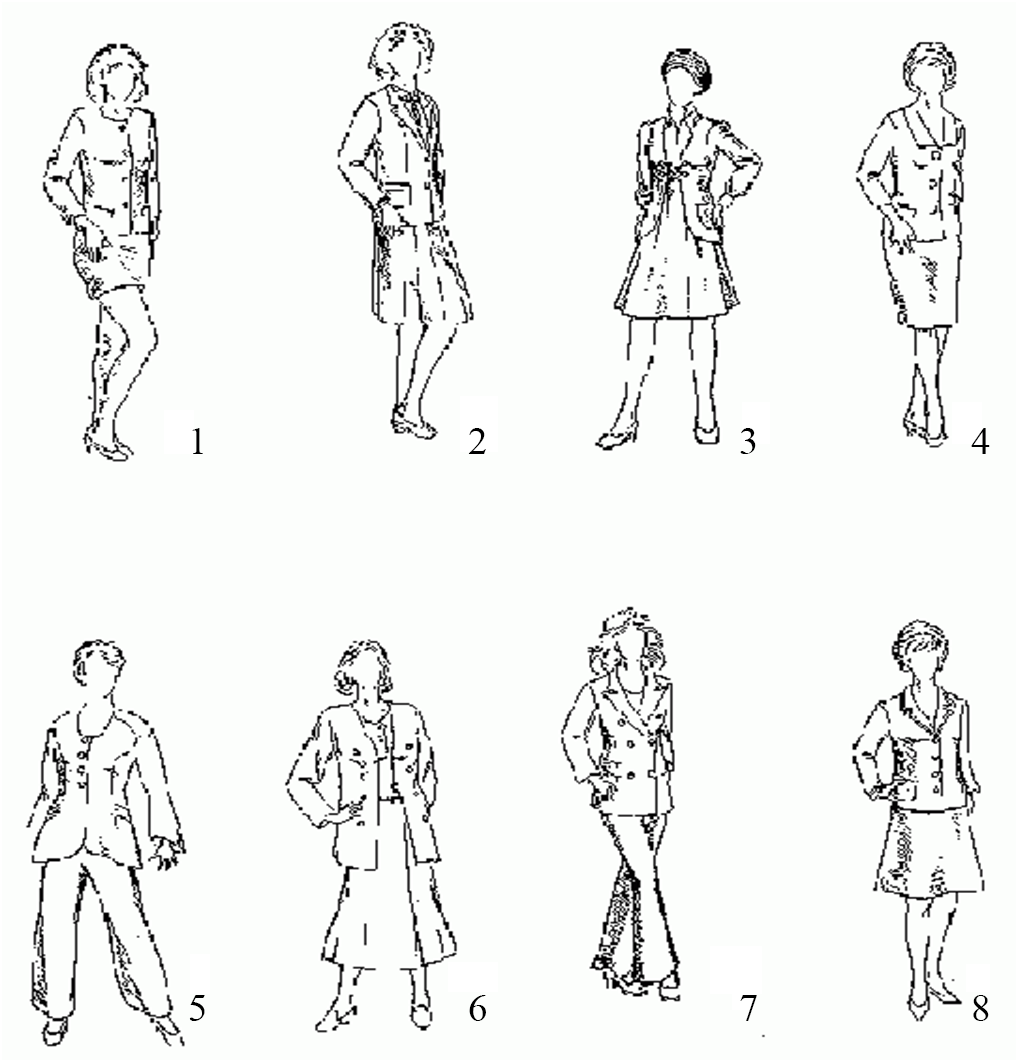
\includegraphics[width=.6\textwidth]{slock_styles}
    \caption{Предлагаемые респонденткам варианты моделей одежды}
    \label{pic:1}
  \end{figure}
  
  Опираясь на результаты анализа данных, можно утверждать, что гипотеза о
  существовании циклов подтвердилась. Продолжительность цикла, в течение
  которого мотивы моделей определенных лет вновь воспроизводятся как модные,
  составляет приблизительно 15--18~лет. Об этом ярко свидетельствует
  периодичность в распределении симпатий и антипатий респонденток к моделям,
  воплощающим характерные черты женской моды 1960--1990-х годов
  (рисунок~\ref{diag:1}).

  \begin{figure}[b!]
    \center
    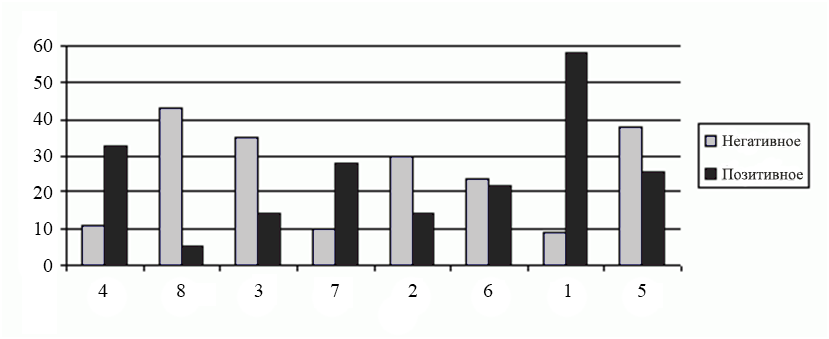
\includegraphics[width=.85\textwidth]{slock_diag-1}
    \caption{Распределение оценок моделей респондентками}
    \label{diag:1}
  \end{figure}
 
  На пике популярности находятся модели~1 (начало 1990-х), 7 (вторая половина
  1970-х) и~4 (первая половина 1960-х годов). Тот факт, что модель~5 (середина
  1990-х) заметно уступает в популярности модели~1, свидетельствует об эффекте
  <<запаздывания>> в распространении модных образцов. Модель, которую журналы
  подают как модную, встречает противоречивую реакцию со стороны потребителей.
  Одними она оценивается как <<неординарная>>, <<забавная>>, <<изящная>>,
  <<элегантная>>, другими как <<безвкусная>>, <<нелепая>>, <<несуразная>>.
  
  Обнаруженная периодичность в предпочтениях респонденток воспроизводится в
  каждом из пяти выделенных поколений. Однако заметны различия между
  поколениями в выборе наиболее привлекательных и наименее привлекательных
  моделей. Эти различия, как представляется, следует объяснять влиянием
  ценностных установок, усвоенных на протяжении формативного периода. Так,
  женщины в возрасте от 23 до 30 лет менее восторженно относятся к модели~1
  (начало 1990-х), чем представительницы поколений 15--22 лет и 31--38 лет.
  Зато они более лояльны к модели~2 (начало 1980-х) и к модели~4 (начало
  1960-х), которые относятся к их формативному периоду. Модель~2 тогда была на
  пике популярности, а модель~4 переживала очередной <<ренессанс>>. Еще одним
  примером, подтверждающим справедливость гипотезы об устойчивости ценностных
  установок, усвоенных в формативный период, является более лояльное, на общем
  негативном фоне, отношение женщин в возрасте 47--55 лет к
  моделям-<<аутсайдерам>>. Модели~8 и~3 воплощают характерные черты моды конца
  1960-х и начала 1970-х годов, т.~е. того времени, когда респонденткам этого
  поколения было 17--25 лет. В отношении модели~4 с поколением 23--30-летних
  солидарно поколение 39--46-летних, на чей формативный период приходится
  другое <<возвращение>> модели~4. Вообще солидарность поколений, разделенных
  характерным периодом 15--18 лет, в отношении к определенным моделям
  достаточно четко прослеживается при сопоставлении числа позитивных~/
  негативных выборов, отнесенных к числу респонденток соответствующего
  поколения (рисунки~\ref{diag:2}--\ref{diag:5}). Приведены диаграммы для
  двух наиболее и двух наименее привлекательных моделей.~\cite{bib:2}

  \begin{figure}[t!]
    \center
    Оценки моделей респондентками различных поколений
    \bigskip
    
    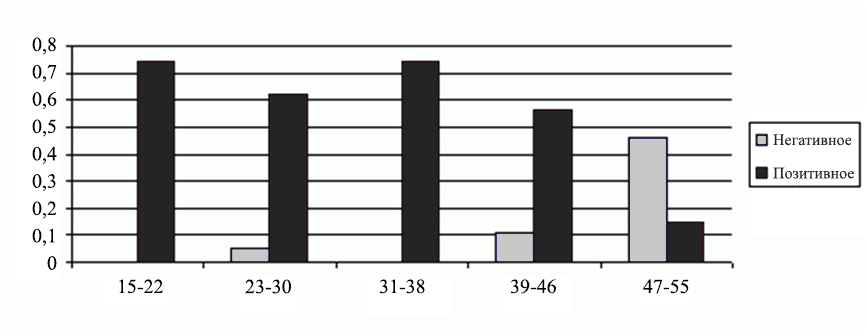
\includegraphics[width=.495\textwidth]{slock_diag-2} \hfill
    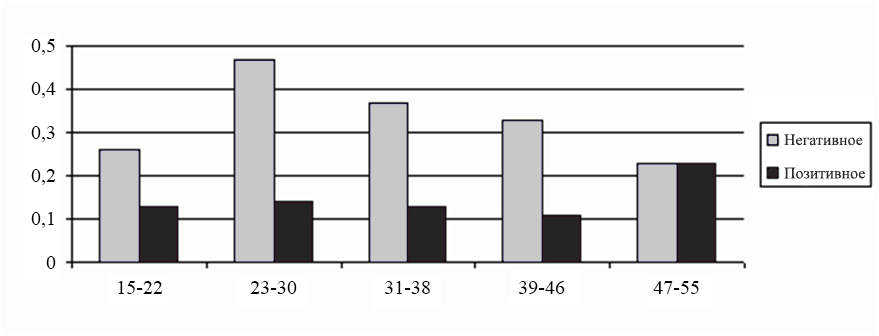
\includegraphics[width=.495\textwidth]{slock_diag-3} \\
    \parbox{.495\textwidth}{\caption{Модель 1} \label{diag:2}} \hfill
    \parbox{.495\textwidth}{\caption{Модель 3} \label{diag:3}}
    
    \bigskip
    \bigskip
    
    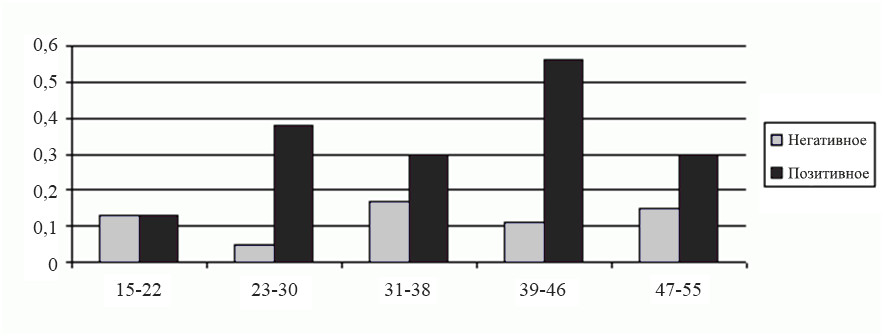
\includegraphics[width=.495\textwidth]{slock_diag-4} \hfill
    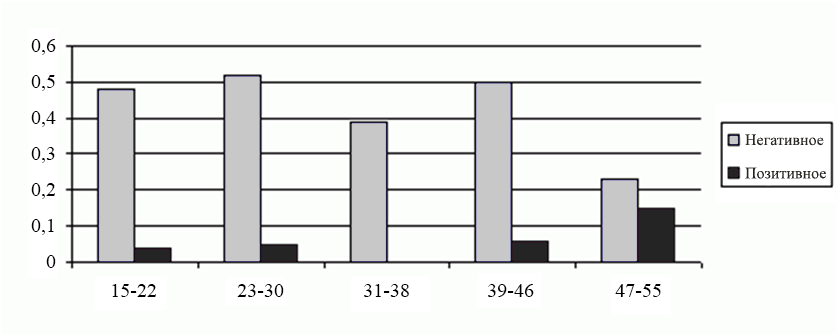
\includegraphics[width=.495\textwidth]{slock_diag-5} \\
    \parbox{.495\textwidth}{\caption{Модель 4} \label{diag:4}} \hfill
    \parbox{.495\textwidth}{\caption{Модель 8} \label{diag:5}}
  \end{figure}

  \section{Мода и стратификация}

  Результаты исследования позволяют по-новому взглянуть на проблему связи моды и
  социальной стратификации. Под стратификацией традиционно понимается устойчивая
  дифференциация общества на группы с неодинаковым доступом к социальным.
  Факторами стратификации являются богатство, власть, престиж, а индикаторами,
  т.~е. показателями~-- уровень дохода, престиж профессии, уровень полномочий в
  организации и~т.~п. В социологии утвердилась практика интерпретации моды как
  специфического индикатора стратификации. Но превращение моды в индустрию
  делает модность составляющей престижа, т.~е. независимой переменной. Роль
  престижа как фактора стратификации в современную эпоху возрастает: если
  когда-то престиж мог быть прямым следствием богатства и власти, то теперь
  зачастую богатство и власть становятся следствием престижа. Например, в
  администрации президента США Р.~Рейгана~-- бывшего киноактера одним из
  министров был бывший профессиональный футболист, списки партийных кандидатов
  на выборах в Государственную Думу в 1995 году изобиловали именами экранных и
  эстрадных звезд, а в Турции в предвыборный список одной из традиционалистских
  партий была включена знаменитая манекенщица, и лидеров партии не остановило
  то, что она специализировалась на демонстрации нижнего белья. Топ-модели и
  спортсмены-звезды успешно <<инвестируют>> свою популярность в рекламный и
  торговый бизнес.
  
  Индустрия моды, <<производя>> модность модели, придает ей социальный статус,
  т.~е. положение, связанное с определенными общественно признаваемыми
  притязаниями на социальные блага. Модность предшествует престижу, престиж~--
  богатству и авторитету. Если даже абстрактная модель (а не реальная стоимость,
  престиж фирменного знака, групповая приверженность) обладает <<виртуальным>>
  социальным статусом, то привлекательность собственно модели, независимо от
  того, приобретают ли и носят ли ее реальные люди, будет легко
  <<конвертироваться>> в престижность <<реального>> социального статуса.
  
  Гипотеза о таком характере связи моды и социальной стратификации проверялась в
  ходе описанного исследования. Предполагалось, что тем моделям, которым
  респондентки будут отдавать предпочтение, они будут приписывать более высокий
  социальный статус. В качестве выражения социального статуса в данном
  исследовании рассматривался престиж того или иного рода деятельности.
  Применительно к женщинам социальный статус определяется двумя факторами: ее
  родом деятельности и родом деятельности ее мужа.
  
  На первом этапе (50~интервью) респонденткам предлагалось назвать наиболее~/
  наименее престижные виды деятельности для женщин и мужчин в современной
  России. Как и следовало ожидать, престижной считается работа в так называемой
  новой экономике~-- в сфере бизнеса и финансов. Банковский работник,
  секретарь-референт, менеджер, бухгалтер составили в сумме абсолютное
  большинство. Среди 50~респонденток их назвали, соответственно, 16, 9, 8, 8
  человек. Кроме того, престижно быть врачом-специалистом (дантистом,
  гинекологом)~-- 11~упоминаний и модельером~-- 10~упоминаний. В современной
  экономической ситуации логично ожидать, что престижность прямо связана с
  доходностью того или иного вида деятельности. Однако идеал престижного занятия
  для женщин сложнее. Весьма характерно определение, данное одной из
  респонденток: <<Престижно работать где-нибудь в офисе с бумагами, быть красиво
  одетой и все время на людях>>. Здесь отчетливо просматривается общая для
  большинства респонденток позиция, свидетельствующая о несводимости
  стратификации к единственному измерению - доходу.
  
  Среди самых непрестижных профессий оказались те, которые связаны с
  малоквалифицированным физическим трудом и малооплачиваемыми должностями в
  общественном секторе экономики. Чаще всего упоминались рабочая (16 раз),
  дворник (12), уборщица (11), педагог в школе и детском саду (11), инженер (8).
  
  Из ответов респонденток ясно видно, что одна и та же профессия может быть
  престижным и непрестижным занятием, в зависимости от того, каков статус
  предприятия, организации в целом. Быть врачом престижно в частной клинике и не
  престижно в районной поликлинике; престижно быть продавцом в фирменном
  магазине и не престижно в ларьке; престижно быть бухгалтером в коммерческой
  фирме и не престижно на заводе.
  
  Сходная картина наблюдается и в том, что касается престижности мужских
  профессий. Респонденткам задавался вопрос о том, за кем престижно быть замужем
  в нынешней России. Престижнее всего быть замужем за бизнесменом - так считают
  более половины респонденток (26 упоминаний). Но и здесь доход не является
  единственным критерием. В представлении женщин престиж мужской работы тесно
  связан с властью. Например, престижно быть замужем за директором,
  руководителем любого рода крупного частного предприятия (11 упоминаний) или
  политическим функционером~-- депутатом, дипломатом, государственным чиновником
  (11). Среди самых непрестижных мужских профессий фигурируют рабочий (15),
  инженер (13), преподаватель (8), дворник (6). Здесь ситуация совершенно
  аналогична ситуации с женскими профессиями. Неоднозначно оценена престижность
  позиций офицеров, врачей-специалистов, научных работников. Их называли в обеих
  категориях, и в целом упоминаний очень мало.
  
  По результатам анализа данных первого этапа исследования были составлены
  списки видов деятельности для мужчин и женщин. На втором этапе исследования
  списки использовались в качестве инструментария. Респонденткам предлагалось
  подобрать к каждой из восьми моделей те профессии из списков, которые наиболее
  подходят возможной обладательнице модели и ее мужу (табл.~\ref{tab:2},
  \ref{tab:3}).
  
  \begin{table}[h!]
    \center
    \small
    \caption{Частота упоминания женских профессий}
    \label{tab:2}
    \begin{tabular}{|C{.16}|*{2}{C{.26}@{ -- }C{.05}|}}                 \hline
      Модель &
        \multicolumn{2}{C{.31}|}{Престижные профессии~--
          количество упоминаний} &
        \multicolumn{2}{C{.31}|}{Непрестижные профессии~--
          количество упоминаний}                                     \\ \hline
      \multirow{4}{*}{1~-- начало~90-х}
        & Секретарь-референт     & 29 & Медсестра               & 8  \\
        & Фотомодель             & 15 & Библиотекарь            & 6  \\
        & Переводчик             & 13 & Уборщица                & 3  \\
        & Менеджер               & 10 & Продавец в ларьке       & 3  \\ \hline
      \multirow{4}{*}{2~-- начало~80-х}
        & Бухгалтер              & 9  & Учитель                 & 23 \\
        & Служащий банка         & 4  & Библиотекарь            & 15 \\
        & Переводчик             & 3  & Воспитатель в д/с       & 8  \\
        & Юрист                  & 3  & Врач-терапевт           & 8  \\ \hline
      \multirow{4}{*}{3~-- начало~70-х}
        & Косметолог             & 8  & Медсестра               & 10 \\
        & Служащий банка         & 4  & Продавец в ларьке       & 8  \\
        & Переводчик             & 3  & Библиотекарь            & 8  \\
        & Юрист                  & 3  & Воспитатель в д/с       & 6  \\ \hline
      \multirow{4}{*}{4~-- начало~60-х}
        & Бухгалтер              & 17 & Учитель                 & 17 \\
        & Депутат                & 15 & Начальник лаб. в НИИ    & 9  \\
        & Служащий банка         & 14 & Библиотекарь            & 7  \\
        & Юрист                  & 11 & Воспитатель в д/с       & 7  \\ \hline
      \multirow{4}{*}{5~-- конец~90-х}
        & Модельер               & 13 & Водитель трамвая        & 8  \\
        & Косметолог             & 11 & Маляр                   & 7  \\
        & Продавец в фирм. маг.  & 7  & Уборщица                & 6  \\
        & Фотомодель             & 6  & Продавец в ларьке       & 4  \\ \hline
      \multirow{4}{*}{6~-- конец~80-х}
        & Бухгалтер              & 10 & Библиотекарь            & 12 \\
        & Юрист                  & 6  & Воспитатель в д/с       & 11 \\
        & Переводчик             & 5  & Инженер                 & 10 \\
        & Служащий банка         & 5  & Начальник лаб. в НИИ    & 8  \\ \hline
      \multirow{4}{*}{7~-- конец~70-х}
        & Переводчик             & 20 & Медсестра               & 7  \\
        & Фотомодель             & 19 & Инженер                 & 4  \\
        & Косметолог             & 10 & Продавец в ларьке       & 4  \\
        & Модельер               & 7  & Водитель трамвая        & 3  \\ \hline
      \multirow{4}{*}{8~-- конец~60-х}
        & Депутат                & 7  & Учитель                 & 13 \\
        & Служащий банка         & 6  & Библиотекарь            & 13 \\
        & Врач-стоматолог        & 5  & Инженер                 & 12 \\
        & Бухгалтер              & 5  & Воспитатель в д/с       & 10 \\ \hline
    \end{tabular}
    
    \medskip
    Источник: Ятина,~Л.~И. Мода глазами социолога: результаты
      эмпирического исследования~/ Л.~И.~Ятина~// Журнал социологии и
      социальной антропологии, том I.~-- 1998.~-- №~2.~-- С.~120--131.
  \end{table}
  
  Анализ полученных данных полностью подтверждает гипотезу о том, что
  привлекательность модели непосредственно связана с престижностью приписываемых
  профессий. Тем моделям, которым респондентки отдают предпочтение, они
  приписывают престижные профессии, привлекательная модель в представлении
  респонденток имеет заведомо высокий <<социальный статус>>, независимо от того,
  носят ли ее реальные люди.
  
  \begin{table}[h!]
    \center
    \small
    \caption{Частота упоминания мужских профессий}
    \label{tab:3}
    \begin{tabular}{|C{.16}|*{2}{C{.26}@{ -- }C{.05}|}}                 \hline
      Модель &
        \multicolumn{2}{C{.31}|}{Престижные профессии~--
          количество упоминаний} &
        \multicolumn{2}{C{.31}|}{Непрестижные профессии~--
          количество упоминаний}                                     \\ \hline
      \multirow{4}{*}{1~-- начало~90-х}
        & Моряк торгового флота  & 18 & Слесарь                 & 5  \\
        & Директор торг. фирмы   & 12 & Врач-хирург в гор. бол. & 4  \\
        & Агент в риелтор. фирме & 12 & Актер театра            & 4  \\
        & Служащий банка         & 9  & Начальник лаб. в НИИ    & 3  \\ \hline
      \multirow{4}{*}{2~-- начало~80-х}
        & Врач-стоматолог        & 7  & Директор школы          & 12 \\
        & Профессор университета & 5  & Инженер                 & 11 \\
        & Чиновник мэрии         & 4  & Мастер по ремонту       & 8  \\
        & Юрист                  & 4  & Офицер ГАИ              & 6  \\ \hline
      \multirow{4}{*}{3~-- начало~70-х}
        & Агент в риелтор. фирме & 7  & Актер театра            & 12 \\
        & Моряк торгового флота  & 7  & Мастер по ремонту       & 5  \\
        & Врач-стоматолог        & 5  & Инженер                 & 5  \\
        & Банковский служащий    & 4  & Слесарь                 & 5  \\ \hline
      \multirow{4}{*}{4~-- начало~60-х}
        & Дипломат               & 16 & Директор школы          & 12 \\
        & Чиновник мэрии         & 16 & Офицер ГАИ              & 7  \\
        & Профессор университета & 10 & Инженер                 & 7  \\
        & Юрист                  & 8  & Начальник лаб. в НИИ    & 5  \\ \hline
      \multirow{4}{*}{5~-- конец~90-х}
        & Моряк торгового флота  & 11 & Актер театра            & 7  \\
        & Менеджер               & 6  & Продавец в ларьке       & 7  \\
        & Агент в риелтор. фирме & 5  & Охранник в фирм. маг.   & 6  \\
        & Дипломат               & 4  & Водитель автобуса       & 5  \\ \hline
      \multirow{4}{*}{6~-- конец~80-х}
        & Профессор университета & 10 & Инженер                 & 15 \\
        & Врач-стоматолог        & 7  & Начальник лаб. в НИИ    & 13 \\
        & Юрист                  & 6  & Врач-хирург в гор. бол. & 11 \\
        & Депутат                & 6  & Директор школы          & 9  \\ \hline
      \multirow{4}{*}{7~-- конец~70-х}
        & Менеджер               & 12 & Актер театра            & 5  \\
        & Директор торг. фирмы   & 11 & Офицер ВМФ              & 5  \\
        & Дипломат               & 10 & Грузчик                 & 4  \\
        & Юрист                  & 9  & Мастер по ремонту       & 4  \\ \hline
      \multirow{4}{*}{8~-- конец~60-х}
        & Служащий банка         & 8  & Инженер                 & 12 \\
        & Чиновник мэрии         & 6  & Токарь                  & 9  \\
        & Профессор университета & 6  & Мастер по ремонту       & 9  \\
        & Врач-стоматолог        & 3  & Директор школы          & 8  \\ \hline
    \end{tabular}
    
    \medskip
    Источник: Ятина,~Л.~И. Мода глазами социолога: результаты
      эмпирического исследования~/ Л.~И.~Ятина~// Журнал социологии и
      социальной антропологии, том I.~-- 1998.~-- №~2.~-- С.~120--131.
  \end{table}
  
  Чем ярче выражена приверженность людей к той или иной модели, тем чаще
  последней приписываются престижные профессии и реже~-- непрестижные, и
  наоборот. Лишь в случае с моделью~5 (конец 1990-х годов) мы сталкиваемся с
  нарушением тенденции. Общая ее оценка негативна. Однако среди ассоциируемых с
  этой моделью женских профессий преобладают престижные: модельер, косметолог,
  продавец в фирменном магазине, фотомодель. Значительно реже данной модели
  приписывались непрестижные профессии: водитель трамвая, маляр, уборщица,
  продавец в ларьке, медсестра. Здесь следует заметить, что мы имеем дело с
  эффектом <<запаздывания>>. Предлагаемая журналами мод модель~5 еще не
  распространилась в обществе. Респондентки знают, что эта модель модна в мире
  моды, но не считают ее таковой для своего жизненного мира. Индустрия моды
  <<увлечена>> этой моделью, но пока не смогла позитивно настроить к ней
  общество, тогда как общество <<увлечено>> индустрией моды как таковой. Именно
  это обстоятельство сказалось на <<социальном статусе>> модели~5. Респондентки
  ориентировались на статус модели в индустрии моды, и баланс в пользу
  престижных профессий предопределен <<вкладом>> профессий, связанных с этой
  сферой.
  
  Полученные результаты нельзя интерпретировать как выявление характерной для
  представителей той или иной профессии манеры одеваться. Очевидно, что
  респондентки ассоциировали одну ценность~-- модность с другой~-- престижностью
  социальной позиции. Рисунки моделей и списки профессий здесь выступают лишь
  как предметные формы ценностей. Проделанный анализ позволяет сделать вывод о
  том, что следование моде повышает в представлении людей социальный статус
  индивида. Таким образом, мода является своего рода фактором стратификации при
  прочих равных условиях. Этот фактор следует учитывать при исследовании проблем
  стратификации современного общества, не преувеличивая и не преуменьшая
  значение моды для социальной дифференциации. В зависимости от ситуации
  исследования, модность может рассматриваться либо в качестве индикатора, либо
  в качестве составляющей престижа как фактора стратификации.~\cite{bib:2}
  
  \section*{Заключение}
  \addcontentsline{toc}{section}{Заключение}

  Мода как потребительская модель предстает как совокупность символов, набор
  знаков или царство кодов. Если в первом случае модные вещи сообщают окружающим
  свойства обладателей, то, став кодами, модные знаки обладают единственным
  означающим императивом~-- <<модностью>>. В разное время этой характеристикой
  наделяется дорогая одежда высших классов, представителей высшего общества или
  одежда других слоев.

  В зависимости от лидера моды, ее движение мыслится по-разному. Оно может быть
  нисходящим, когда модные образцы курсируют от высших слоев к более низким, что
  показывают Веблен или Зиммель. Если циркуляция модных образцов характеризуется
  отсутствием однонаправленности, его характеризуют как диффузное,~-- такой
  способ распространения моды описывает Блумер. В отдельных случаях мода
  распространяется снизу вверх, такое движение можно назвать восходящим. Та или
  иная характеристика моды, возникающая в дискурсе, в соответствии с основной
  идеей, появляется вслед за изменениями в обществе.

  В настоящее время ярко выделяется влияние общественного сознания на отдельных
   индивидов в области моды, одежды которую мы носим, вещами которыми мы
  пользуемся. Но также при анализе исторических данных можно заметить, что мода
  циклична. В отличии от первобытного времени, в котором одежда имела лишь
  практическую функцию, в современном обществе она приобрела и множество других
  функций. Костюм отражает культурное наследие общества, историческое наследие,
  этнические особенности. Но также одежда современного человека это способ
  самовыражения, общения, передачи информации и~др.
  
  Из истории я заметила, что люди придают одежде символический смысл, и в ходе
  моей работы такая гипотеза подтвердилась. Для современного человека одежда
  имеет более сакральный смысл, чем для наших далеких предков.

  \newpage

  \renewcommand{\bibname}{Список использованной литературы}
  \begin{thebibliography}{9}
    \addcontentsline{toc}{section}{Список использованной литературы}
    \bibitem{bib:0} Определение понятия моды [Электронный ресурс].~--
      Режим доступа:\\
      \url{http://trixx.ru/index.php/istoriya-mody/
        98-opredelenie-ponyatiya-mody}
    \bibitem{bib:1} Одежда и социология [Электронный ресурс].~--
      Режим доступа:\\
      \url{http://psyfactor.org/lib/dresscode.htm}
    \bibitem{bib:2} Ятина,~Л.~И. Мода глазами социолога: результаты
      эмпирического исследования~/ Л.~И.~Ятина~// Журнал социологии и
      социальной антропологии, том I.~-- 1998.~-- №~2.~-- С.~120--131.
    \bibitem{bib:3} Гофман,~А.~Б. Мода и люди. Новая теория моды и модного
      поведения. 3-е изд.~/ А.~Б.~Гофман.~-- СПб.:~Питер, 2004.~-- 208~с: ил.
    \bibitem{bib:4} Бодрийяр,~Ж. Символический обмен и смерть~/
      Ж.~Бодрийяр.~-- М.:~Добросвет, 2000.~-- 387~с.
    \bibitem{bib:5} Бодрийяр,~Ж. Система вещей~/
      Ж.~Бодрийяр.~-- М.:~Рудомино, 2001.~-- 220~с.
  \end{thebibliography}

\end{document}
